\documentclass[a4paper,11pt,oneside]{memoir}

% Castellano
\usepackage[spanish]{babel}
\selectlanguage{spanish}
\usepackage[utf8]{inputenc}
\usepackage{placeins}

\RequirePackage{booktabs}
\RequirePackage[table]{xcolor}
\RequirePackage{xtab}
\RequirePackage{multirow}

% Links
\usepackage[colorlinks]{hyperref}
\hypersetup{
	allcolors = {red}
}

% Ecuaciones
\usepackage{amsmath}

% Rutas de fichero / paquete
\newcommand{\ruta}[1]{{\sffamily #1}}

% Párrafos
\nonzeroparskip


% Imagenes
\usepackage{graphicx}
\newcommand{\imagen}[2]{
	\begin{figure}[!h]
		\centering
		\includegraphics[width=0.9\textwidth]{#1}
		\caption{#2}\label{fig:#1}
	\end{figure}
	\FloatBarrier
}

\newcommand{\imagenflotante}[2]{
	\begin{figure}%[!h]
		\centering
		\includegraphics[width=0.9\textwidth]{#1}
		\caption{#2}\label{fig:#1}
	\end{figure}
}



% El comando \figura nos permite insertar figuras comodamente, y utilizando
% siempre el mismo formato. Los parametros son:
% 1 -> Porcentaje del ancho de página que ocupará la figura (de 0 a 1)
% 2 --> Fichero de la imagen
% 3 --> Texto a pie de imagen
% 4 --> Etiqueta (label) para referencias
% 5 --> Opciones que queramos pasarle al \includegraphics
% 6 --> Opciones de posicionamiento a pasarle a \begin{figure}
\newcommand{\figuraConPosicion}[6]{%
  \setlength{\anchoFloat}{#1\textwidth}%
  \addtolength{\anchoFloat}{-4\fboxsep}%
  \setlength{\anchoFigura}{\anchoFloat}%
  \begin{figure}[#6]
    \begin{center}%
      \Ovalbox{%
        \begin{minipage}{\anchoFloat}%
          \begin{center}%
            \includegraphics[width=\anchoFigura,#5]{#2}%
            \caption{#3}%
            \label{#4}%
          \end{center}%
        \end{minipage}
      }%
    \end{center}%
  \end{figure}%
}

%
% Comando para incluir imágenes en formato apaisado (sin marco).
\newcommand{\figuraApaisadaSinMarco}[5]{%
  \begin{figure}%
    \begin{center}%
    \includegraphics[angle=90,height=#1\textheight,#5]{#2}%
    \caption{#3}%
    \label{#4}%
    \end{center}%
  \end{figure}%
}
% Para las tablas
\newcommand{\otoprule}{\midrule [\heavyrulewidth]}
%
% Nuevo comando para tablas pequeñas (menos de una página).
\newcommand{\tablaSmall}[5]{%
 \begin{table}
  \begin{center}
   \rowcolors {2}{gray!35}{}
   \begin{tabular}{#2}
    \toprule
    #4
    \otoprule
    #5
    \bottomrule
   \end{tabular}
   \caption{#1}
   \label{tabla:#3}
  \end{center}
 \end{table}
}

%
% Nuevo comando para tablas pequeñas (menos de una página).
\newcommand{\tablaSmallSinColores}[5]{%
 \begin{table}[H]
  \begin{center}
   \begin{tabular}{#2}
    \toprule
    #4
    \otoprule
    #5
    \bottomrule
   \end{tabular}
   \caption{#1}
   \label{tabla:#3}
  \end{center}
 \end{table}
}

\newcommand{\tablaApaisadaSmall}[5]{%
\begin{landscape}
  \begin{table}
   \begin{center}
    \rowcolors {2}{gray!35}{}
    \begin{tabular}{#2}
     \toprule
     #4
     \otoprule
     #5
     \bottomrule
    \end{tabular}
    \caption{#1}
    \label{tabla:#3}
   \end{center}
  \end{table}
\end{landscape}
}

%
% Nuevo comando para tablas grandes con cabecera y filas alternas coloreadas en gris.
\newcommand{\tabla}[6]{%
  \begin{center}
    \tablefirsthead{
      \toprule
      #5
      \otoprule
    }
    \tablehead{
      \multicolumn{#3}{l}{\small\sl continúa desde la página anterior}\\
      \toprule
      #5
      \otoprule
    }
    \tabletail{
      \hline
      \multicolumn{#3}{r}{\small\sl continúa en la página siguiente}\\
    }
    \tablelasttail{
      \hline
    }
    \bottomcaption{#1}
    \rowcolors {2}{gray!35}{}
    \begin{xtabular}{#2}
      #6
      \bottomrule
    \end{xtabular}
    \label{tabla:#4}
  \end{center}
}

%
% Nuevo comando para tablas grandes con cabecera.
\newcommand{\tablaSinColores}[6]{%
  \begin{center}
    \tablefirsthead{
      \toprule
      #5
      \otoprule
    }
    \tablehead{
      \multicolumn{#3}{l}{\small\sl continúa desde la página anterior}\\
      \toprule
      #5
      \otoprule
    }
    \tabletail{
      \hline
      \multicolumn{#3}{r}{\small\sl continúa en la página siguiente}\\
    }
    \tablelasttail{
      \hline
    }
    \bottomcaption{#1}
    \begin{xtabular}{#2}
      #6
      \bottomrule
    \end{xtabular}
    \label{tabla:#4}
  \end{center}
}

%
% Nuevo comando para tablas grandes sin cabecera.
\newcommand{\tablaSinCabecera}[5]{%
  \begin{center}
    \tablefirsthead{
      \toprule
    }
    \tablehead{
      \multicolumn{#3}{l}{\small\sl continúa desde la página anterior}\\
      \hline
    }
    \tabletail{
      \hline
      \multicolumn{#3}{r}{\small\sl continúa en la página siguiente}\\
    }
    \tablelasttail{
      \hline
    }
    \bottomcaption{#1}
  \begin{xtabular}{#2}
    #5
   \bottomrule
  \end{xtabular}
  \label{tabla:#4}
  \end{center}
}



\definecolor{cgoLight}{HTML}{EEEEEE}
\definecolor{cgoExtralight}{HTML}{FFFFFF}

%
% Nuevo comando para tablas grandes sin cabecera.
\newcommand{\tablaSinCabeceraConBandas}[5]{%
  \begin{center}
    \tablefirsthead{
      \toprule
    }
    \tablehead{
      \multicolumn{#3}{l}{\small\sl continúa desde la página anterior}\\
      \hline
    }
    \tabletail{
      \hline
      \multicolumn{#3}{r}{\small\sl continúa en la página siguiente}\\
    }
    \tablelasttail{
      \hline
    }
    \bottomcaption{#1}
    \rowcolors[]{1}{cgoExtralight}{cgoLight}

  \begin{xtabular}{#2}
    #5
   \bottomrule
  \end{xtabular}
  \label{tabla:#4}
  \end{center}
}




\graphicspath{ {./img/} }

% Capítulos
\chapterstyle{bianchi}
\newcommand{\capitulo}[2]{
	\setcounter{chapter}{#1}
	\setcounter{section}{0}
	\chapter*{#2}
	\addcontentsline{toc}{chapter}{#2}
	\markboth{#2}{#2}
}

% Apéndices
\renewcommand{\appendixname}{Apéndice}
\renewcommand*\cftappendixname{\appendixname}

\newcommand{\apendice}[1]{
	%\renewcommand{\thechapter}{A}
	\chapter{#1}
}

\renewcommand*\cftappendixname{\appendixname\ }

% Formato de portada
\makeatletter
\usepackage{xcolor}
\newcommand{\tutor}[1]{\def\@tutor{#1}}
\newcommand{\course}[1]{\def\@course{#1}}
\definecolor{cpardoBox}{HTML}{E6E6FF}
\def\maketitle{
  \null
  \thispagestyle{empty}
  % Cabecera ----------------
\noindent
\includegraphics[width=\textwidth]{cabecera}\vspace{1cm}%
  \vfill
  % Título proyecto y escudo informática ----------------
  \colorbox{cpardoBox}{%
    \begin{minipage}{.8\textwidth}
      \vspace{.5cm}\Large
      \begin{center}
      \textbf{TFG del Grado en Ingeniería Informática}\vspace{.6cm}\\
      \textbf{\LARGE\@title{}}
      \end{center}
      \vspace{.2cm}
    \end{minipage}

  }%
  \hfill\begin{minipage}{.20\textwidth}
    
\includegraphics[width=\textwidth]{escudoInfor}
  \end{minipage}
  \vfill
  % Datos de alumno, curso y tutores ------------------
  \begin{center}%
  {%
    \noindent\LARGE
    Presentado por \@author{}\\ 
    en Universidad de Burgos --- \@date{}\\
    Tutor: \@tutor{}\\
  }%
  \end{center}%
  \null
  \cleardoublepage
  }
\makeatother


% Datos de portada
\title{título del TFG \\Documentación Técnica}
\author{nombre alumno}
\tutor{nombre tutor}
\date{\today}

\begin{document}

\maketitle



\cleardoublepage



%%%%%%%%%%%%%%%%%%%%%%%%%%%%%%%%%%%%%%%%%%%%%%%%%%%%%%%%%%%%%%%%%%%%%%%%%%%%%%%%%%%%%%%%



\frontmatter


\clearpage

% Indices
\tableofcontents

\clearpage

\listoffigures

\clearpage

%\listoftables

%\clearpage

\mainmatter

\appendix

\apendice{Plan de Proyecto}

\section{Introducción}

A lo largo de este apéndice se va a presentar tanto la evolución temporal que ha seguido el proyecto durante su realización como aquellos aspectos de viabilidad que puedan afectar al trabajo si se desease continuar con él en un futuro.

\section{Planificación temporal}

En esta sección vamos a presentar un resumen de lo que ha sido la realización del proyecto. 

El desarrollo del proyecto se ha llevado a cabo mediante el uso de metodologías ágiles, realizando reuniones periódicas con los tutores para debatir sobre el desarrollo del trabajo y definir nuevos objetivos. Estas reuniones se han realizado, salvo excepciones, de manera bisemanal, y suponían el fin de un periodo de trabajo (\textit{sprint}) y el comienzo del siguiente. Durante estas reuniones, además, se presentaba el trabajo realizado durante la última iteración.

Con el fin de no expandir más de lo necesario este anexo, solo se presentará una breve descripción del trabajo realizado en sprint del proyecto. Información más amplia sobre cada uno de los hitos y/o tareas puede encontrarse en la sección \textit{Issues} del repositorio del proyecto, donde los hitos formarán un \textit{issue} y las tareas, así como conversaciones entre los miembros del proyecto, pueden verse recogidas dentro de dicho \textit{issue}.

\subsection{Sprint 1 [29/09/15-13/10/15]}

Partiendo de un estado de desconocimiento de la tecnología a utilizar durante el desarrollo, se ha invertido gran parte del tiempo en aprender el funcionamiento de Spark y la terminología del área de trabajo.

Igualmente, se realiza el despliegue de todos los materiales necesarios para el desarrollo. Algunos de ellos no fueron necesarios para iteraciones siguientes, como Python o Hadoop, y han sido eliminados más adelante. Además, el despliegue se realizó por duplicado, al encontrar problemas con la ejecución de Spark en el sistema operativo Windows.

Finalmente, se presentan dos pequeños programas (uno en Java y otro en Scala) para comprobar el funcionamiento de Spark y poder decidir el lenguaje a usar durante la etapa de desarrollo.

\subsection{Sprint 2 [13/10/15-29/10/15]}

Se selecciona Scala como lenguaje de programación y comenzamos a aprender las bases de dicho programa.

Como objetivo principal de este sprint se plantea realizar una comparativa entre el tiempo de ejecución entre Weka y Spark con el algoritmo Naive Bayes. Todo ello genera una serie de hitos, definidos en las líneas sucesivas.

Se busca una serie de conjuntos de datos con diferentes características de tamaño/número de atributos, que además cumplan una serie de condiciones, como la ausencia de valores nulos. A la mayoría de los conjuntos seleccionados, pese a todo, hubo que pre procesarlos para que pudiesen funcionar sin problemas con Spark.

Se genera una pequeña clase lanzadora en Spark para poder lanzar y medir nuestros experimentos. Del mismo modo se realizan pequeñas modificaciones en el código de Weka para poder realizar correctamente mediciones.

Además, el comienzo de la documentación forzó al aprendizaje de \LaTeX.

Finalmente, se terminó el sprint con la entrega del algoritmo en Scala utilizado para las mediciones y un informe con la explicación, resultados y conclusiones de la comparación Weka-Spark.

\subsection{Sprint 3 [29/10/15-19/11/15]}

A partir de este momento comenzamos a centrarnos en otro de los objetivos principales del proyecto: la implementación de algoritmos de selección de instancias.
 
Se implementa una primera versión del LSHIS y se generan diferentes métodos para realizar labores como la lectura de datos. Es la primera implementación con cierta complicación que realizamos tanto en Scala como para Spark, por lo que este hito ya se plantea con una carga de trabajo importante.

Al final del sprint contamos con una implementación de una primera versión funcional del algoritmo LSHIS.

\subsection{Sprint 4 [19/11/15-10/12/15]}

Se reestructura todo el código de la iteración anterior, creando nuevos paquetes, clases y relaciones de herencia. Además, se empieza a utilizar herramientas para el control estático de la calidad del código, lo que fuerza algunos cambios para adaptarnos a los estándares fijados.

El propio algoritmo LSHIS sufre una mejora, permitiendo ahora ejecutarlo con uno o varios componentes OR.

Se comienza la implementación del algoritmo DemoIS, pero queda suspendida a la espera de contar con una implementación paralela del algoritmo \textit{k}-Nearest Neighbors (\textit{k}NN).

Igualmente frenada por esta espera del algoritmo \textit{k}NN, se plantea una comparación entre nuestra implementación LSHIS y la ya realizada en Weka, aunque nunca llega a producirse dentro de este sprint.

Se crea una máquina virtual con todos los materiales necesarios para el despliegue y distribución sencilla de nuestra aplicación.

Al finalizar este sprint contamos con una versión mejorada del algoritmo LSHIS, una mejor estructuración de nuestro código y un entorno para la fácil distribución de nuestro trabajo.

\subsection{Sprint 5 [10/12/15-22/12/15]}

Se implementa de manera completa el algoritmo DemoIS. Esto obliga a la creación de algunos otros componentes como el algoritmo \textit{k}NN, cuya implementación paralela no pudimos conseguir.

Se realizan pruebas sobre nuestro algoritmo LSHIS. Dichas pruebas generan un número considerable de problemas y, finalmente, cuando conseguimos realizar las mediciones, éstas arrojan malos resultados.

La máquina virtual sufre modificaciones para facilitar la ejecución del proyecto dentro de la misma.

Tras el sprint, podemos mostrar un nuevo algoritmo de selección de instancias y una máquina virtual mejor preparada para permitir la ejecución del proyecto.

\subsection{Sprint 6 [22/12/15-08/01/16]}

Se realiza una primera implementación de la interfaz gráfica, que acaba por afectar a prácticamente la totalidad de la biblioteca, aunque nunca de manera sustancial.

Las pruebas sobre nuestros algoritmos siguen siendo problemáticas y continuamos trabajando sobre ello. Durante este periodo se encuentran una serie de errores que afectaban a la manera en la que medíamos el tiempo de ejecución, así como unos errores en los algoritmos de Weka con los que intentábamos comparar nuestros resultados.

Finalmente, comenzamos a estudiar como lanzar nuestra ejecución en algún servicio de computación en la nube, pero no llegamos a finalizar la tarea al considerar más prioritario acabar con los problemas descritos anteriormente.

Por lo tanto, al terminar esta etapa contamos con una nueva manera de ejecutar nuestra aplicación (mediante la interfaz gráfica) y una serie de errores importantes corregidos, tanto en nuestra aplicación como en la librería de Weka facilitada.

\subsection{Sprint 7 [08/01/16-25/01/16]}

Se realiza una nueva iteración sobre nuestra implementación de los algoritmos, esta vez centrada en mejorar el tiempo de ejecución de los mismos, que continua siendo muy elevado con respecto a Weka. Es algo que se resolverá en este sprint.

Habiendo solventado todos los problemas, comenzamos, de nuevo, a realizar pruebas sobre el rendimiento de nuestro trabajo.

Igualmente, iniciamos otra tarea que había quedado suspendida, el despliegue del proyecto en un clúster real, lanzándolo finalmente en dos servicios diferentes: Google Beta Dataproc \cite{dataprocSoft} y un servicio clúster con el que contaba la Universidad de Burgos.

Durante este periodo también se trabaja en una gran refactorización del código, cuya calidad había disminuido considerablemente con todos los cambios introducidos en el sprint anterior.

Al finalizar esta iteración contamos con unos algoritmos que han demostrado funcionar correctamente y los resultados de una serie de comparativas que hemos realizado sobre nuestras implementaciones.

\subsection{Sprint 8 [25/01/16-05/02/16]}

Entre este periodo y el anterior, se mantienen una serie de ejecuciones de nuestros algoritmos en el servicio clúster con el que cuenta la universidad, pero acaban cancelándose por problemas con los nodos.

Se realizan pequeñas modificaciones en el código en vista a mejorar su calidad o corregir algún comportamiento indeseado.

Para terminar, se prepara la versión final de todos los materiales necesarios para la presentación del proyecto al finalizar este último sprint.


\section{Estudio de viabilidad}

El trabajo presentado a lo largo de este proyecto podría enfocarse de dos maneras distintas en esta sección: por un lado, podemos hablar de la viabilidad de los algoritmos implementados. Por otro, de las bases que este proyecto podría sentar para construir una librería con algoritmos de selección de instancias que corran en paralelo.

Sobre el primer punto, la viabilidad de los algoritmos, podemos basarnos en su rendimiento (estudiado en el anexo \ref{anexo:Pruebas}) para concluir que, aunque una de nuestras implementaciones (LSHIS) no aporta una gran mejoría en cuanto a tiempo de ejecución se refiere, la otra (DemoIS) puede llegar fácilmente a mejorar los tiempos de respuesta de su predecesora. Además, ambos algoritmos están pensados para su ejecución sobre grandes conjuntos de datos, algo que no pueden soportar las versiones anteriores de estos algoritmos y que nos proporciona una ventaja fundamental en un ambiente donde cada vez existen un mayor número de datos que analizar.

Sobre el proyecto como una base para formar una librería, supondría, no solo trabajar en un área en continua expansión, sino comenzar en un momento en el que no existen otras grandes librerías que trabajen con Spark, lo que nos proporciona una gran flexibilidad para orientar el proyecto a donde se estime conveniente.

En lo que se refiere a aspectos de viabilidad es interesante referirse también al posible futuro de la tecnología en la que se basa el proyecto: Spark.

Aunque Apache Spark es una librería cuya versión inicial se presentó a mediados de 2014, ha gozado de buena acogida desde entonces, siendo actualmente uno de los proyectos mejor valorados de la fundación Apache Software Foundation y uno de los más activos \cite{ApacheContributions}. Igualmente, podemos observar en la gráfica \ref{fig:img/anexo/spark_StackOverflow} como el interés por esta tecnología ha crecido en un corto periodo de tiempo para equipararse en interés a muchas de las soluciones ya existentes en el mercado. Nos encontramos, por lo tanto, operando con una tecnología que promete seguir desarrollándose gracias a la aceptación con la que ha sido recibida.

\imagen{img/anexo/spark_StackOverflow}{Evolución del interés por Apache Spark en la plataforma Stack Overflow \cite{SparkAnalysisRedMonk}.}


\subsection{Viabilidad económica}

Aunque este proyecto nunca ha sido enfocado a un aspecto de comercialización inmediata, podemos ver un escenario favorable en el sentido económico.

La minería de datos es un ámbito del que se espera rápida y fuerte expansión. Podemos observar en la gráfica \ref{fig:img/anexo/Forbes_big_data} como la intención de muchas de las empresas es la de continuar apostando por la inversión en minería de datos, que ha llegado a convertirse en una prioridad para una gran cantidad de empresas de sectores muy diversos \cite{forbesBigData}.

\imagen{img/anexo/Forbes_big_data}{Interés de las empresas por apostar por el Big Data (2014) \cite{forbesBigData}.}

Un campo en expansión puede proporcionarnos un buen terreno para obtener la rentabilidad económica, pero para ello necesitamos contar con alguna ventaja competitiva que nos permita diferenciarnos del competidor. Podemos destacar la modernidad de la tecnología utilizada, que, al estar enfocada al llamado \textit{big data}, consigue realizar tareas que soluciones anteriores no podían resolver en un tiempo prudencial. Además, dentro del tipo de aplicacaciones que ofertan esta posibilidad, podemos destacar de Spark la capacidad de utilizar memoria para agilizar las operaciones.

En referencia a los servicios sobre los que ejecutar nuestra aplicación, nos encontramos en un punto en el que no es necesario contar con una enorme inversión inicial para hacerse con todo el hardware necesario para conseguir un rápido análisis de datos (clúster con varios nodos, gran capacidad de memoria RAM, etc.). Actualmente, estos servicios pueden contratarse a empresas que ya cuentan con todos estos recursos (tales como Google y su servicio Google Cloud), pagando solo por el uso que hacemos de ellos, lo que abre todavía más el mercado de empresas que podrían permitirse el uso de un clúster para ejecutar este tipo de tareas de minería de datos.

\textbf{Clientes objetivo y licencias de distribución}

Aunque, como se ha mencionado, nunca se ha tenido en mente enfocar este producto a ningún aspecto de comercialización concreto, podemos distinguir dos grúpos de clientes sobre los que podría trabajarse:

\begin{itemize}
\item \textbf{Educación e investigación:} Al igual que otras alternativas existentes en el mercado (como Weka \cite{WekaSoft} o KEEL \cite{KEELSoft1, KEELSoft2}), nuestro proyecto podría abordar el área de la educación desde una nueva perspectiva: la creación de una librería de algoritmos de minería de datos paralelos.

En esta situación, se distribuiría el producto utilizando la licencia GNU GPL (\textit{GNU General Public License}), por la ventaja que esto podría proporcionar para estudiar, modificar o distribuir nuevos materiales a partir de nuestro producto. Además, este tipo de licencia garantizaría que cualquier material generado como una iteración del proyecto siga manteniendo la misma licencia y, por lo tanto, pueda seguir siendo útil en el área de la educación.

\item \textbf{Empresas que manejen grandes volúmenes de datos:} Aunque la minería de datos es algo que parece estar cogiendo fuerza en muchas áreas, nuestra ventaja competitiva reside en la capacidad para tratar problemas de \textit{big data} (grandes conjuntos de datos) de manera eficiente. Es por ello que nuestro objetivo deberían ser aquellas organizaciones, por lo general de gran tamaño, que tengan el problema de tratar con tal cantidad de datos.

En este supuesto, el proyecto podría orientarse para actuar como una capa intermedia entre la empresa y un servicio de computación de la nube. Por las características ya mencionadas de estos servicios de computación, nuestro servicio debería ofrecerse de manera que el usuario adquiriese derecho a uso por un periodo de tiempo limitado, pudiendo renovar o cancelar la suscripción pasado ese tiempo y haciendo más asequible el precio final. Cabe destacar que esta es una situación que el trabajo presentado, más orientado a la investigación, no está preparado para afrontar en la etapa actual, por lo que no se teorizará más sobre el posible desarrollo económico.

\end{itemize}

\subsection{Viabilidad legal}

En lo que se refiere a aspectos legales, este trabajo no se encuentra en problemática con ningún aspecto que pudiese considerarse de dudosa o nula legalidad, dado que se ha centrado en la implementación y pruebas de diferentes algoritmos.

Con respecto a la minería de datos, el problema más cuestionable es la protección de los datos analizados y la privacidad que se puede ofrecer  si dichos datos hacen referencia a una persona o entidad concreta. Sin embargo, en su estado actual, nuestra aplicación no gestiona ni tienen interés en gestionar ningún aspecto de este terreno. 




\apendice{Especificación de Requisitos}


\section{Introducción}

A lo largo de este apéndice, vamos a hacer referencia a todo lo relacionado con los objetivos del proyecto, indicando apropiadamente las metas y cuáles han sido los requisitos que han guiado el desarrollo de nuestro trabajo.

\section{Objetivos generales}

Podemos definir dos claros objetivos con los que se comenzó el proyecto:
\begin{itemize}

\item La implementación de una serie de algoritmos de selección de instancias que puedan ser ejecutados utilizando el nuevo paradigma de programación paralela que nos ofrece Spark. Estos algoritmos son: \textit{Localy sensitive hashing instance selection} (LSHIS) \cite{LSHISPaper} y \textit{Democratic instance selection} (DemoIS) \cite{DemoISPaper}

\item La comparativa entre el rendimiento de las soluciones secuenciales de minería de datos frente a las nuevas soluciones de ejecución paralela que han surgido recientemente. Esta tarea se llevará a cabo utilizando una librería ya existente (Weka) para realizar ejecuciones que sigan el modelo secuencial, y Spark para realizar ejecuciones paralelas.

Las mediciones deberán están enfocadas en dos sentidos: una comparación general del rendimiento entre Spark y Weka, y la comparación concreta de nuestras implementaciones, definidas en el punto anterior, sobre aquellas que ya estén creadas para la librería Weka.
\end{itemize}

Igualmente, y conforme el proyecto iba avanzando, se consideró añadir una nueva serie de objetivos, de importancia menor, a nuestra aplicación:

\begin{itemize}
\item La creación de una interfaz gráfica más amigable y visual que no solo facilite el uso de todo el material generado, sino que permita, además, definir baterías de experimentos para ser ejecutados al instante o en una máquina diferente.
\item El despliegue del proyecto en el entorno donde está pensado para ser ejecutado: un clúster con diferentes nodos y múltiples unidades de procesamiento.
\end{itemize}

\section{Catalogo de requisitos}

\subsection{Requisitos funcionales}

\begin{itemize}

\item \textbf{RF-1} La aplicación ha de permitir el lanzamiento mediante línea de comandos, de ejecuciones de minería de datos que consten de un algoritmo de selección de instancias y un clasificador.
	\begin{itemize}
		\item \textbf{RF-1.1} Se podrá indicar si se desea o no realizar la medición del tiempo de filtrado.
		\item \textbf{RF-1.2} Se podrán indicar opciones para la correcta lectura del conjunto de datos. Esto implica indicar donde estará el atributo de clase y si el fichero contiene o no cabecera.
		\item \textbf{RF-1.3} Se deberá indicar un algoritmo de selección de instancias, junto con su configuración, al iniciar la tarea.
		\item \textbf{RF-1.4} Se deberá indicar un algoritmo de clasificación, junto con su configuración, al iniciar la tarea.
		\item \textbf{RF-1.5} Se podrá indicar si se desea realizar validación cruzada en las ejecuciones. En caso de no indicarse nada, existirá una opción por defecto de usar el 10\% del conjunto de datos incial como test para nuestras pruebas.
		\item \textbf{RF-1.6} Se generará un fichero con el resumen de la ejecución: reducción del algoritmo de selección de instancias, precisión del clasificador y, si ha sido requerido, el tiempo de filtrado.
	\end{itemize}

\item \textbf{RF-2} La aplicación ha de permitir, vía interfaz gráfica, el lanzamiento de ejecuciones o baterías de ejecuciones que consten de un algoritmo de selección de instancias y un clasificador.
	\begin{itemize}
		\item \textbf{RF-2.1} Se podrán seleccionar algunas de las opciones de lanzamiento de Spark (ruta al directorio de instalación de Spark, ruta al nodo maestro, número de núcleos, número de ejecutores y memoria de cada ejecutor).
		\item \textbf{RF-2.2} Se podrán elegir uno o más conjuntos de datos, aunque en cada ejecución solo se use uno.
		\item \textbf{RF-2.3} Se podrá elegir y configurar uno o más algoritmos de preprocesamiento, aunque en cada ejecución solo se use uno.
		\item \textbf{RF-2.4} Se deberá seleccionar y configurar un algoritmo de clasificación.
		\item \textbf{RF-2.5} Se podrán configurar las opciones para realizar una validación cruzada.
		\item \textbf{RF-2.6} Se almacenará un fichero por cada lanzamiento con los datos de reducción y precisión de la ejecución.
	\end{itemize}

\item \textbf{RF-3} La aplicación ha de permitir, mediante la interfaz gráfica, definir ejecuciones o baterías de ejecuciones y exportar estos experimentos en un archivo .zip con los materiales necesarios.
	\begin{itemize}
		\item \textbf{RF-3.1} Se podrán seleccionar algunas de las opciones de lanzamiento de Spark (ruta al directorio de instalación de Spark, ruta al nodo maestro, número de núcleos, número de ejecutores y memoria de cada ejecutor).
		\item \textbf{RF-3.2} Se podrán elegir uno o más conjuntos de datos, junto con sus opciones para una correcta lectura de los mismos. Se utilizará un conjunto de datos por ejecución
		\item \textbf{RF-3.3} Se podrá elegir y configurar uno o más algoritmos de preprocesamiento, usando uno por ejecución.
		\item \textbf{RF-3.4} Se podrá seleccionar y configurar un algoritmo de clasificación.
		\item \textbf{RF-3.5} Se deberá generar un archivo .zip que contenga un script para ejecutar la batería de ejecuciones, junto con todos los conjuntos de datos necesarios para las ejecuciones.
	\end{itemize}

\item \textbf{RF-4} Debe existir una sección destinada a explicar el funcionamiento de la interfaz gráfica.

\end{itemize}

\subsection{Requisitos no funcionales}

\begin{itemize}

\item \textbf{RNF-1} La implementación no ha de tener problemas para correr en paralelo o en sistemas distribuidos formados por varios nodos.

\item \textbf{RNF-2} El código ha de cumplir con una serie de medidas estáticas de calidad.

\item \textbf{RNF-3} Los resultados de reducción y precisión generados por nuestros algoritmos de selección de instancias han de ser similares a los generados por la implementación secuencial de dichos algoritmos.

\item \textbf{RNF-4} La aplicación ha de poder lanzarse en algún de los servicios de computación que ofrecen la posibilidad de correr Spark, concretamente Google Cloud Dataproc.

\item \textbf{RNF-5} Ha de proporcionarse un sistema que facilite el uso de nuestra aplicación y la generación de baterías de ejecuciones sin necesidad de recurrir a la consola de comandos.

\end{itemize}

\section{Especificación de requisitos}

\subsection{Diagrama de casos de uso}

	\begin{figure}[!h]
		\centering
		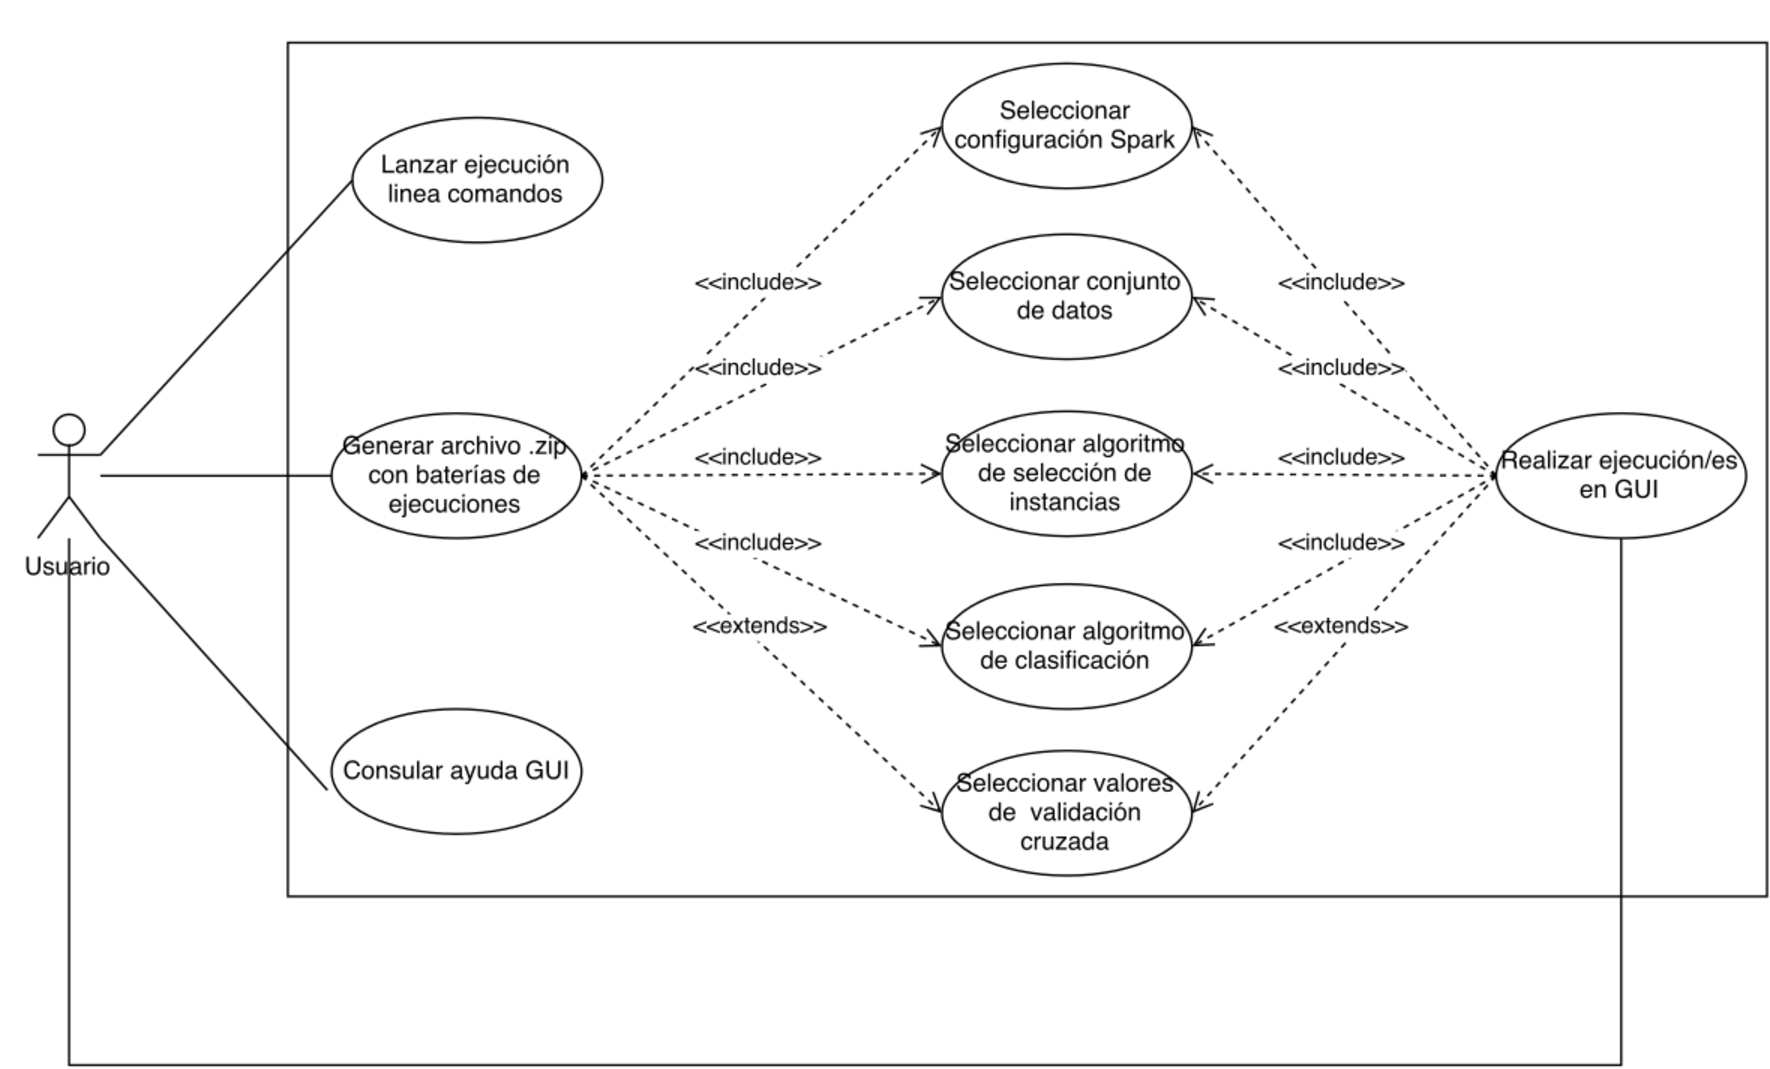
\includegraphics[width=1.0\textwidth]{img/anexo/diagrama_casos_de_uso}
		\caption{Diagrama de casos de uso.}\label{fig:img/anexo/diagrama_casos_de_uso}
	\end{figure}

%\imagen{img/anexo/diagrama_casos_de_uso}{Diagrama de casos de uso.}

 
\subsection{Casos de uso}
 
\begin{table}
  \begin{center}
   \begin{tabular}{|>{\cellcolor[gray]{0.8}} L{3cm} | L{9cm} |}
    \hline
    Caso de uso & Lanzar ejecución - Línea de comandos\\
    \hline
    Versión & 1.0 \\
    \hline
    Autor & Alejandro González Rogel \\
    \hline
    Requisitos & RF-1\newline
		RF-1.1\newline
		RF-1.2\newline
		RF-1.3\newline
		RF-1.4\newline
		RF-1.5\newline
		RF-1.6\\
    \hline
    Descripción & El usuario puede realizar la invocación, por línea de comandos, de un nueva tarea que implique un selector de instancias y un clasificador. Para ello necesitará aportar, además, una lista de parámetros que permitan la configuración de todos los componentes involucrados.\\
    \hline
    Precondiciones & Ninguna \\
    \hline
    Acciones & 1. El usuario realiza el lanzamiento de la aplicación mediante consola de comandos usando el script ``spark-submit'' proporcionado por Spark. \newline
    2. La aplicación realiza la ejecución. \newline
    \hspace{1em} 2.1 Se muestra periodicamente, en mensajes por consola, el punto de la ejecución en el que nos encontramos. \newline
    \hspace{1em} 2.2 La aplicación escribe los resultados de la ejecución en un fichero.\newline
    \hspace{1em} 2.3 La aplicación muestra un último mensaje indicando la correcta ejecución.\\
    \hline
    Postcondiciones & Ningua \\
    \hline
    Excepciones & Los parámetros introducidos en la invocación del programa son erróneos. Se paralizará la ejecución y se informará mediante un mensaje por consola de comandos si este fuese el caso. \\
    \hline
    Importancia & Alta \\
    \hline
   \end{tabular}
   \caption{Caso de uso ``Lanzar ejecución - Línea de comandos''}
   \label{tabla:casoUso1}
  \end{center}
 \end{table} 
 
 
\begin{table}
  \begin{center}
   \begin{tabular}{|>{\cellcolor[gray]{0.8}} L{3cm} | L{9cm} |}
    \hline
    Caso de uso & Realizar ejecución/es GUI\\
    \hline
    Versión & 1.0 \\
    \hline
    Autor & Alejandro González Rogel \\
    \hline
    Requisitos & 
    		RF-2\newline
    		RF-2.1\newline
		RF-2.2\newline
		RF-2.3\newline
		RF-2.4\newline
		RF-2.5\newline
		RF-2.6\\
    \hline
    Descripción & Mediante el uso de la interfaz gráfica, el usuario puede programar una o varias ejecuciones y lanzarlas en el momento.\\
    \hline
    Precondiciones & El usuario ha iniciado la interfaz gráfica. \\
    \hline
    Acciones & 1. El usuario completa los campos de opciones comunes de Spark. \newline
    			   2. El usuario indica una o varias configuraciones de Spark \newline
    			   3. El usuario indica uno o varios conjuntos de datos \newline
    			   4. El usuario selecciona uno o varios selectores de instancias. \newline
    			   5. El usuario selecciona un clasificador. \newline
    			   6. El usuario puede indicar opciones para la validación cruzada (opcional). \newline
    			   7. El usuario presiona un botón para ejecutar las tareas programadas. \newline
    			   8. La aplicación informa cuando se finalice la operación.
    			   \\
    \hline
    Postcondiciones & Los resultados de la ejecución han sido almacenados en un fichero de texto en la ruta correspondiente. \\
    \hline
    Excepciones & Ninguna \\
    \hline
    Importancia & Baja \\
    \hline
   \end{tabular}
   \caption{Caso de uso ``Realizar ejecución/es GUI''}
   \label{tabla:casoUso2}
  \end{center}
 \end{table} 
 
 
\begin{table}
  \begin{center}
   \begin{tabular}{|>{\cellcolor[gray]{0.8}} L{3cm} | L{9cm} |}
    \hline
    Caso de uso & Generar archivo .zip con baterías de ejecuciones\\
    \hline
    Versión & 1.0 \\
    \hline
    Autor & Alejandro González Rogel \\
    \hline
    Requisitos & 
    		RF-2\newline
    		RF-2.1\newline
		RF-2.2\newline
		RF-2.3\newline
		RF-2.4\newline
		RF-2.5\newline
		RF-2.6\\
    \hline
    Descripción & Mediante el uso de la interfaz gráfica, el usuario puede programar una o varias ejecuciones y generar un archivo de extensión .zip que contendrá un script de lanzamiento y todos los conjuntos de datos necesarios para la ejecución.\\
    \hline
    Precondiciones & El usuario ha iniciado la interfaz gráfica. \\
    \hline
    Acciones & 1. El usuario completa los campos de opciones generales de Spark. \newline
    			   2. El usuario indica una o varias configuraciones de Spark \newline
    			   3. El usuario indica uno o varios conjuntos de datos \newline
    			   4. El usuario selecciona uno o varios selectores de instancias. \newline
    			   5. El usuario selecciona un clasificador. \newline
    			   6. El usuario puede indicar opciones para la validación cruzada (opcional). \newline
    			   7. El usuario presiona un botón para generar el archivo zip. \newline
    			   8. La aplicación informa cuando se finalice la operación.
    			   \\
    \hline
    Postcondiciones & Se ha generado un archivo de extensión .zip \\
    \hline
    Excepciones & Ninguna \\
    \hline
    Importancia & Media \\
    \hline
   \end{tabular}
   \caption{Caso de uso ``Generar archivo .zip con baterías de ejecuciones''}
   \label{tabla:casoUso3}
  \end{center}
 \end{table}  
 
 
 \begin{table}
  \begin{center}
   \begin{tabular}{|>{\cellcolor[gray]{0.8}} L{3cm} | L{9cm} |}
    \hline
    Caso de uso & Seleccionar configuración Spark\\
    \hline
    Versión & 1.0 \\
    \hline
    Autor & Alejandro González Rogel \\
    \hline
    Requisitos & RF-2\newline
    				 RF-2.1\newline
    				 RF-3\newline
    				 RF-3.1 \\
    \hline
    Descripción & El usuario puede indicar una configuración de Spark rellenando un conjunto de campos de texto. \\
    \hline
    Precondiciones & El usuario ha iniciado la interfaz gráfica.\\
    \hline
    Acciones & 1. El usuario ha presionado un botón para añadir una nueva configuración de Spark. \newline
    			   2. La aplicación muestra un nuevo diálogo. \newline
    			   3. El usuario rellena todos los campos mostrados en el nuevo diálogo. \newline
    			   4. El usuario presiona un botón para aceptar la nueva configuración.  \\
    \hline
    Postcondiciones & Una nueva configuración ha de haberse añadido a la lista de configuraciones. \\
    \hline
    Excepciones & Ninguna \\
    \hline
    Importancia & Baja \\
    \hline
   \end{tabular}
   \caption{Caso de uso ``Seleccionar configuración Spark''}
   \label{tabla:casoUso5}
  \end{center}
 \end{table}
 
  \begin{table}
  \begin{center}
   \begin{tabular}{|>{\cellcolor[gray]{0.8}} L{3cm} | L{9cm} |}
    \hline
    Caso de uso & Seleccionar conjunto de datos\\
    \hline
    Versión & 1.0 \\
    \hline
    Autor & Alejandro González Rogel \\
    \hline
    Requisitos & RF-2\newline
    				 RF-2.2\newline
    				 RF-3\newline
    				 RF-3.2 \\
    \hline
    Descripción & El usuario puede indicar un fichero que contenga un conjunto de datos así como algunos parámetros que permitan su lectura. \\
    \hline
    Precondiciones & El usuario ha iniciado la interfaz gráfica.\\
    \hline
    Acciones & 1. El usuario ha presionado un botón para añadir un nuevo conjunto de datos. \newline 
    2. La aplicación muestra un nuevo diálogo. \newline
    			   3. El usuario selecciona el botón para buscar en los archivos del sistema un conjunto de datos. Alternativamente, puede escribirlo manualmente. \newline
    			   4. El usuario cumplimenta todos los campos restantes mostrados en el diálogo. \newline
    			   5. El usuario presiona un botón para aceptar la nueva configuración. \\
    \hline
    Postcondiciones & Un nuevo conjunto de datos, junto con sus opciones de lectura, ha de haberse añadido a la lista de conjuntos de datos. \\
    \hline
    Excepciones & Ninguna \\
    \hline
    Importancia & Baja \\
    \hline
   \end{tabular}
   \caption{Caso de uso ``Seleccionar conjunto de datos''}
   \label{tabla:casoUso6}
  \end{center}
 \end{table}
 
 
   \begin{table}
  \begin{center}
   \begin{tabular}{|>{\cellcolor[gray]{0.8}} L{3cm} | L{9cm} |}
    \hline
    Caso de uso & Seleccionar algoritmo de selección de instancias\\
    \hline
    Versión & 1.0 \\
    \hline
    Autor & Alejandro González Rogel \\
    \hline
    Requisitos & RF-2\newline
    				 RF-2.3\newline
    				 RF-3\newline
    				 RF-3.3 \\
    \hline
    Descripción & El usuario puede seleccionar un algoritmo de selección de instancias de entre las posibles opciones y configurarlo para su ejecución. \\
    \hline
    Precondiciones & El usuario ha iniciado la interfaz gráfica.\\
    \hline
    		Acciones & 1.El usuario ha presionado el botón para añadir un nuevo selector de instancias.  \newline
    		
    		2. La aplicación muestra un nuevo diálogo. \newline
    		3. El usuario selecciona, tras pulsar el botón de selección, el filtro que desea. \newline
    		4. La aplicación añade nuevos campos al diálogo.
    		5. El usuario cumplimenta los nuevos campos mostrados en el diálogo. \newline
    		6. El usuario presiona un botón para aceptar la nueva configuración. \\
    \hline
    Postcondiciones & Un nuevo selector de instancias, junto con su configuración, ha de haberse añadido a la lista de conjuntos de datos. \\
    \hline
    Excepciones & Ninguna \\
    \hline
    Importancia & Baja \\
    \hline
   \end{tabular}
   \caption{Caso de uso ``Seleccionar algoritmo de selección de instancias''}
   \label{tabla:casoUso7}
  \end{center}
 \end{table}
 
    \begin{table}
  \begin{center}
   \begin{tabular}{|>{\cellcolor[gray]{0.8}} L{3cm} | L{9cm} |}
    \hline
    Caso de uso & Seleccionar algoritmo de clasificación.\\
    \hline
    Versión & 1.0 \\
    \hline
    Autor & Alejandro González Rogel \\
    \hline
    Requisitos & RF-2\newline
    				 RF-2.4\newline
    				 RF-3\newline
    				 RF-3.4 \\
    \hline
    Descripción & El usuario puede seleccionar un algoritmo de clasificación y configurarlo para su ejecución. \\
    \hline
    Precondiciones & El usuario ha iniciado la interfaz gráfica.\\
    \hline
    		Acciones & 1. El usuario presiona el botón que permite seleccionar entre los diferentes clasificadores posibles. \newline
    		2. El usuario selecciona un clasificador.\newline
    		3. La aplicación genera nuevos campos con las opciones de configuración del clasificador.\newline
    		4. El usuario rellena los campos con las opciones de configuración.    \\ 			
    \hline
    Postcondiciones & Ninguna\\
    \hline
    Excepciones & Ninguna \\
    \hline
    Importancia & Baja \\
    \hline
   \end{tabular}
   \caption{Caso de uso ``Seleccionar algoritmo de clasificación''}
   \label{tabla:casoUso8}
  \end{center}
 \end{table}
 
 
     \begin{table}
  \begin{center}
   \begin{tabular}{|>{\cellcolor[gray]{0.8}} L{3cm} | L{9cm} |}
    \hline
    Caso de uso & Seleccionar valores de validación cruzada.\\
    \hline
    Versión & 1.0 \\
    \hline
    Autor & Alejandro González Rogel \\
    \hline
    Requisitos & RF-2\newline
    				 RF-2.5\newline
    				 RF-3\newline
    				 RF-3.5 \\
    \hline
    Descripción & El usuario puede indicar una configuración de validación cruzada con la que realizar las ejecuciones. \\
    \hline
    Precondiciones & El usuario ha iniciado la interfaz gráfica.\\
    \hline
    		Acciones & 1. El usuario marca la opción que habilita la validación cruzada. \newline
    		2. El usuario cumplimenta los campos de configuración de la validación cruzada.\\
    \hline
    Postcondiciones & Ninguna\\
    \hline
    Excepciones & Ninguna \\
    \hline
    Importancia & Baja \\
    \hline
   \end{tabular}
   \caption{Caso de uso ``Seleccionar valores de validación cruzada''}
   \label{tabla:casoUso9}
  \end{center}
 \end{table}
 
 
 
 \begin{table}
  \begin{center}
   \begin{tabular}{|>{\cellcolor[gray]{0.8}} L{3cm} | L{9cm} |}
    \hline
    Caso de uso & Consultar ayuda GUI\\
    \hline
    Versión & 1.0 \\
    \hline
    Autor & Alejandro González Rogel \\
    \hline
    Requisitos & RF-4 \\
    \hline
    Descripción & El usuario puede consultar el funcionamiento de la interfaz gráfica mediante un botón de ayuda proporcionado en dicha interfaz.\\
    \hline
    Precondiciones & Se ha iniciado la interfaz gráfica. \\
    \hline
    Acciones & 1. El usuario presiona sobre el botón de ayuda en la interfaz. \newline
    				2. La aplicación muestra una nueva ventana con la ayuda.\\
    \hline
    Postcondiciones & Ninguna \\
    \hline
    Excepciones & Ninguna \\
    \hline
    Importancia & Baja \\
    \hline
   \end{tabular}
   \caption{Caso de uso ``Consultar ayuda GUI''}
   \label{tabla:casoUso4}
  \end{center}
 \end{table}
\apendice{Especificación de diseño}

\section{Introducción}

\section{Diseño de datos}

\section{Diseño procedimental}

\section{Diseño arquitectónico}



\apendice{Documentación técnica de programación}


\section{Introducción}

En este apéndice se van a describir todos aquellos aspectos que se consideren de interés para una persona que desee continuar el desarrollo del proyecto o quiera obtener un conocimiento más avanzado del mismo.

\section{Estructura de directorios}

A continuación se va a hacer mención a la funcionalidad de cada una de las carpetas que conforman el árbol de directorios de nuestro proyecto:

\begin{itemize}
	\item \textbf{src:} Carpeta destinada a almacenar el código fuente la aplicación.
	\begin{itemize}
		\item \textbf{main/scala:} Este directorio contendrá todos los ficheros fuente que estén escritos en Scala. Al no haberse usado ningún otro lenguaje ni contar con clases para realizar pruebas, este es el único directorio de la carpeta ``src''.
	\end{itemize}
	\item \textbf{resources:} Carpeta destinada a almacenar todos aquellos elementos que, sin ser código, también son necesarios para la ejecución del programa. Aquí podríamos incluir fichero .xml, html, imágenes o cualquier otro fichero multimedia, etc.
	\begin{itemize}
		\item \textbf{gui:} Contiene todos los recursos utilizados por la interfaz gráfica.
		\item \textbf{loggerStrings:} Almacena ficheros de texto con sentencias que pueden ser utilizadas por los diferentes \textit{logger} en diferentes clases de nuestro programa.
	\end{itemize}
	\item \textbf{target:} Contiene los archivos resultantes de aplicar alguna operación de Apache Maven sobre el proyecto (compilación, empaquetado o generación de documentación). Para más información al respecto visitar la sección \ref{subsec:compilacion}, situada en este mismo anexo.
	\begin{itemize}
		\item \textbf{site/scaladocs:} Ruta que contiene la documentación, generada por Scaladoc, de las clases del proyecto.
	\end{itemize}
\end{itemize}


\section{Manual del programador}

A lo largo de esta sección vamos a describir diferentes tareas que, si bien no se refieren directamente a la ejecución del programa, pueden conducir a un manejo más avanzado del mismo.

Antes de proceder es necesario comprender y haber realizado el proceso de instalación de todos los componentes mencionados en la sección \ref{sec:Instalacion}, independientemente de si esos componentes han sido marcados como opcionales o no para el usuario normal.

\subsection{Configurando Spark para guardar información sobre ejecuciones}\label{subsec:configurandoSpark}

Con la configuración por defecto, Spark apenas almacena información sobre las ejecuciones realizadas, pudiendo acceder a parámetros sobre la ejecución solo mientras el programa está corriendo. A lo largo de esta sección explicaremos que es posible modificar este comportamiento y la manera de lograrlo.

Lo primero que necesitamos es modificar algunas propiedades de Spark. En su carpeta de configuración  (\textit{\$SPARK\_HOME/conf}) debemos buscar un fichero por nombre ``spark-defaults.conf''. Si es la primera vez que realizamos este tipo de operaciones es posible que este fichero no exista, haciendo necesario crearlo nosotros mismos o renombrar el fichero ``spark-defaults.conf.template'' que actúa de ejemplo y está situado en la misma carpeta.

Sea cual sea la opción elegida, en nuestro fichero de configuración ``spark-defaults.conf'' escribiremos las siguientes líneas:

\begin{lstlisting}[basicstyle=\small]
spark.eventLog.enabled	true
spark.eventLog.dir	    /opt/spark-1.5.1/logs/exec-logs
spark.history.fs.logDirectory /opt/spark-1.5.1/logs/exec-logs
\end{lstlisting}

La primera línea es obligatoria y no admite cambios. Las dos siguientes sirven para indicar el fichero donde deseamos almacenar la información de las ejecuciones. La ruta seleccionada es indiferente, pero es necesario destacar dos aspectos:
\begin{itemize}
\item Las dos rutas indicadas han de ser iguales.
\item Las rutas han de apuntar a un directorio existente. Si indicamos una ruta inexistente Spark no generará los directorios que falten, sino que emitirá un error cuando intentemos ejecutar una aplicación y esta quiera guardar sus datos de ejecución. Es por ello que, en el caso concreto de la configuración ofrecida como ejemplo, deberíamos crear la carpeta ``exec-logs'' en  \textit{/opt/spark-1.5.1/logs} antes de proceder.
\end{itemize}

Con esto, deberíamos contar con toda la información de nuestras ejecuciones aun después de que estas hayan acabado. Será en la siguiente sección cuando hablaremos de cómo acceder a todos estos datos para su posterior análisis.


\subsection{Monitorización y análisis}\label{subsec:monitorizacion}

Un aspecto clave en el desarrollo de aplicaciones para \textit{big data} es el de controlar y analizar el rendimiento de los algoritmos. Para ello, vamos a explicar en la siguiente sección como acceder a este tipo de información. No es objetivo de este anexo, sin embargo, explicar toda la información analizable ni la manera en la que ésta se organiza.

Antes de continuar, es necesario indicar que toda esta información proporcionada aquí corresponde a la manera de analizar una aplicación ejecutada en el modo \textit{Standalone} de Spark (ver sección \ref{subsec:modosDespliegueSpark} para más información). Si Spark se ejecutase usando algún administrador de clústeres el modo de acceder a la información podría ser distinto dependiendo del software usado. Igualmente, si ejecutamos en modo local no existe una manera de acceder a los datos de análisis una vez la aplicación ha finalizado su ejecución.

Con todo, comenzaremos contemplando la posibilidad de observar la ejecución de un programa mientras éste está todavía en ejecución. Esto puede hacerse accediendo, mediante el navegador, a la ruta \url{http://localhost:4040} (suponemos que nuestra máquina es el nodo maestro). Podemos ver un ejemplo de la página inicial en la imagen \ref{fig:img/anexo/pantalla_4040}. Esta información solo estará disponible mientras la aplicación lanzada siga ejecutando, y toda la información que podemos ver será borrada si no hemos seguido los pasos descritos en la anterior subsección.

\imagen{img/anexo/pantalla_4040}{Ejemplo de monitorización de una aplicación en marcha.}

Suponiendo que queremos realizar un análisis de todas las aplicaciones que han sido lanzadas en la red de nodos en modo \textit{Standalone}, podemos hacerlo consultado la dirección \url{http://localhost:8080}. Además de información referente a nuestro clúster, podemos observar un listado de aplicaciones ejecutadas o en ejecución, a cuya información se puede acceder pulsando sobre cualquiera de ellas (ver imagen \ref{fig:img/anexo/pantalla_8080}).

\imagen{img/anexo/pantalla_8080}{Pantalla de inicio de un clúster Standalone.}

De nuevo, la ruta indicada ruta es válida si únicamente estamos trabajando en la máquina local o somos el nodo maestro de la red. Igualmente, volvemos a recordar que hemos tenido que habilitar la opción de Spark para guardar información de las ejecuciones.

Por último, si deseamos acceder a toda la información de ejecuciones guardada en nuestra máquina, independiente de si continuamos formando parte de una red de nodos o hemos sido el nodo maestro de varias redes, podemos accederlo iniciando el servicio ``History Server'' y accediendo a la ruta (\url{http://localhost:18080/}), donde se nos mostrará un listado con todas las aplicaciones ejecutadas de las que se tiene información. Para iniciar el servicio mencionado, desde consola de comandos, debemos escribir el comando:

\begin{lstlisting}[language=bash]
$ $SPARK_HOME/sbin/start-history-server.sh
\end{lstlisting}

Podemos ver un ejemplo del histórico de ejecuciones en la imagen \ref{fig:img/anexo/pantalla_18080}.

\imagen{img/anexo/pantalla_18080}{Ejemplo de la interfaz del servidor de históricos.}

\section{Compilación, instalación y ejecución}

A lo largo de esta sección vamos a hablar de todos los pasos necesarios para poder trabajar sobre el código del proyecto. Esto incluye la instalación de diferentes componentes, la configuración del entorno de desarrollo y la comprensión de la herramienta Apache Maven como administrador en labores como la compilación.

\subsection{Instalación}

Si deseamos trabajar sobre el código del proyecto, además de necesitar todos los materiales definidos en la sección \ref{sec:Instalacion} vamos a necesitar los definidos en este apartado.

\subsubsection{Scala 2.11.7}
Aunque podemos descargar la última versión de Scala desde la página oficial (\url{http://www.scala-lang.org/}), la descarga que se nos ofrece por defecto es un archivo .tar.gz que nos obligaría a realizar toda la instalación manualmente (suponiendo que estamos en un sistema Ubuntu como el utilizado durante el proyecto).

Por ello, vamos a realizar la instalación mediante un archivo .deb (paquete Debian) que también puede ser utilizado por nuestro sistema y que nos ahorrará realizar la instalación manualmente. Podemos acceder al repositorio que guarda este paquete desde un navegador (\url{http://www.scala-lang.org/files/archive/}) o descargarlo mediante el siguiente comando:

\begin{lstlisting}[language=bash]
$ wget www.scala-lang.org/files/archive/scala-2.11.7.deb
\end{lstlisting}

Independientemente del método seguido, una vez tengamos el archivo en nuestro ordenador ejecutamos el siguiente comando desde la carpeta que contenga el paquete .deb:

\begin{lstlisting}[language=bash]
$ sudo dpkg -i scala-2.11.7.deb
\end{lstlisting}

Si todo ha salido correctamente, una vez termine de ejecutarse la orden anterior podemos ejecutar el comando \textit{scala -version} y esperar una salida similar a esta:

\begin{lstlisting}[language=bash]
$ scala -version
Scala code runner version 2.11.7 -- Copyright 2002-2013
\end{lstlisting}

Recordar que, en el caso de utilizar cualquier otra versión de Scala, esta tiene que ser compatible con la versión Java que se encuentre instalada. Por ejemplo, Java 8 solo puede ser utilizado a partir de versiones 2.11 y será obligatorio a partir de la versión de Scala 2.12. \cite{Scala2.12Roadmap}

\subsubsection{Scala IDE}

Scala IDE es el entorno de desarrollo utilizado durante el proyecto.

Descargaremos la  última versión disponible del producto desde su página oficial: \url{http://scala-ide.org/}

Dentro de las posibles descargas que podemos seleccionar, elegiremos aquella que esté destinada a nuestro sistema operativo, en nuestro caso concreto, ``Linux - 64 bits''. Al descargar esta herramienta, en realidad estamos descargando el entorno de desarrollo Eclipse (\url{https://eclipse.org/}) con una serie de \textit{plugins} añadidos, entre los que destaca el llamado Scala IDE.

Una vez descargado, descomprimiremos el archivo en la ruta \textit{/opt}. Mediante línea de comandos podemos hacerlo utilizando la siguiente sentencia:

\begin{lstlisting}
$ cd /opt/ && sudo tar -zxvf \
~/Downloads/scala-SDK-4.2.0-vfinal-2.11-\
linux.gtk.x86_64.tar.gz
\end{lstlisting}

Recuerde que el código puede cambiar dependiendo del nombre del archivo que sea descargado o del directorio donde se encuentre.

\subsection{Importando el proyecto en Scala IDE}


Suponiendo que se ha seguido la instalación del entorno de desarrollo mencionado (Scala IDE) seguiremos los siguientes pasos para importar y ejecutar nuestro proyecto desde el propio programa.

Primero de todo, para importar el código a nuestro lugar de trabajo debemos dirigirnos al menú superior, opción ``File'' y, de entre las alternativas del menú desplegable, seleccionar ``Import''. Alternativamente también podemos abrir el menú desplegable haciendo clic derecho sobre el panel de nombre ``Package explorer'', situado generalmente a la izquierda de la pantalla.

Veremos un nuevo diálogo similar al mostrado en la figura \ref{fig:img/anexo/existing_maven_projects}, donde seleccionaremos, entre todas las opciones, aquella que diga ``Existing Maven Projects''. Posteriormente, presionamos sobre el botón ``Next'' para continuar.

\imagen{img/anexo/existing_maven_projects}{Diálogo para seleccionar un médoto de importación en Eclipse IDE.}

En el nuevo diálogo presionaremos sobre el botón ``Browse'' para indicar el directorio principal de nuestro proyecto. Si todo es correcto, una vez seleccionemos la carpeta que deseemos el resultado debería ser similar al mostrado en la imagen \ref{fig:img/anexo/proyecto_importado}.

\imagen{img/anexo/proyecto_importado}{Diálogo para importar un proyecto al entorno Eclipse IDE.}

Pulsamos sobre el botón de finalizar y, si todo ha salido correctamente, deberíamos poder ver nuestro proyecto en el menú lateral izquierdo, tal como muestra \ref{fig:img/anexo/paquete_importado}

\imagen{img/anexo/paquete_importado}{Paquete importado en el menú lateral.}


\subsection{Ejecutando el proyecto en Scala IDE}

Como puede observarse en el manual del usuario (\ref{sec:manualUsuario}) el lanzamiento de una aplicación en Spark se realiza mediante un script que proporciona el propio Spark y en el cual se pueden indicar ciertos parámetros de ejecución. Por ello, para el lanzamiento del programa desde Eclipse hemos de modificar añadir algún fragmento de código que genere una configuración de Spark que, en cualquier otro método de lanzamiento, es creada por el script utilizado.

Para ello hemos de modificar un fragmento de código en la clase \textit{ISClassExec} del paquete \textit{launcher.execution}, tal y como puede verse en \ref{lst:codigoSpark} y \ref{lst:codigoSpark2}


\begin{lstlisting}[language=Java,tabsize=4,frame = single,caption=Código para la ejecución del programa mediante el script ``spark-sumbit''. ,captionpos=b,label=lst:codigoSpark]
val sc = new SparkContext()
\end{lstlisting}

\begin{lstlisting}[language=Java,tabsize=4,frame = single,caption=Ejemplo de código para la ejecución del programa desde Eclipse. ,captionpos=b,label=lst:codigoSpark2]
	val master = "local[2]"
    val sparkConf =
  	  new SparkConf().setMaster(master)
  	  .setAppName("Prueba_Eclipse")
    val sc = new SparkContext(sparkConf)
\end{lstlisting}

Ahora, debemos indicar, de manera manual, cuál será la clase principal que deseamos lanzar. Es posible que esto cambie de acuerdo al tipo de ejecución que queremos realizar (lanzar la interfaz gráfica o un experimento de Spark), pero los pasos a seguir son idénticos.

Desde la pantalla de Scala IDE nos dirigiremos al menú superior, presionamos sobre ``Run'' y seleccionamos la opción ``Run configurations''. Esto abrirá una nueva ventana similar a la mostrada en la figura \ref{fig:img/anexo/run_configurations}.

Presionando dos veces sobre el texto ``Scala application'', en el menú izquierdo, podremos generar una nueva configuración para el proyecto. Allí rellenaremos los campos requeridos, con especial interés al campo ``Main Class'', que deberá escribirse manualmente porque el entorno no detecta ninguna de las clases principales de los proyectos. En nuestro caso, ese campo siempre será \textit{launcher.ExperimentLauncher} para lanzar experimentos y \textit{gui.SparkISGUI} para lanzar la interfaz gráfica.


\imagen{img/anexo/run_configurations}{Ventana de configuración de ejecuciones en Scala IDE.}


Finalmente, si deseamos introducir argumentos al iniciar una ejecución, podemos hacerlo desde la pestaña ``Arguments'', en la ventana anterior, rellenando el campo ``Program arguments'' con la información que deseemos (ver ejemplo en \ref{fig:img/anexo/arguments_configuration})

\imagen{img/anexo/arguments_configuration}{Ventana de configuración de ejecuciones en Scala IDE - Argumentos.}


Con todo definido, podemos presionar sobre el botón ``Run'' para comenzar a ejecutar nuestro programa.

Para posteriores ejecuciones no necesitaremos volver a definir de nuevo todo el proceso, sino que la opción será guardada y podrá ser accedida de manera sencilla seleccionándola desde el menú desplegable que proporciona el botón de ejecutar en el menú superior de Eclipse (ver figura \ref{fig:img/anexo/menu_superior_eclipse}).

	\begin{figure}[!h]
		\centering
		
\includegraphics[width=0.4\textwidth]{img/anexo/menu_superior_eclipse}
		\caption{Fragmento del menú superior de Scala IDE.}\label{fig:img/anexo/menu_superior_eclipse}
	\end{figure}
	
Si tenemos configurado el entorno para no realizar la compilación automática de las clases o hemos modificado algún recurso, debe realizarse una acción anterior al lanzamiento de cualquier ejecución. Desde la ventana principal del entorno de desarrollo, haremos clic con el botón derecho sobre la carpeta de nuestro proyecto, ``Run as'', ``Maven build''. Se nos abrirá una ventana similar a la mostrada en la figura \ref{fig:img/anexo/eclipse_maven}.
	
	\imagen{img/anexo/eclipse_maven}{Ventana de configuración de Maven.}
	
Simplemente, necesitamos escribir en el campo de texto ``Goals'' los objetivos ``clean package'' y presionar sobre el botón ``Run''. Esto debería realizar la compilación de todo el proyecto desde el entorno de desarrollo.

	
	\subsection{Compilación}\label{subsec:compilacion}

Para realizar la labor de compilación vamos a necesitar del software Apache Maven, cuya instalación ha sido indicada en \ref{subsec:instalaMaven}. Una vez contemos con este requisito la operación será prácticamente automática.

Desde consola nos dirigimos al directorio raíz donde esté situado el proyecto. Una vez allí, ejecutamos el comando siguiente:

\begin{lstlisting}[language=bash]
$ mvn clean package
\end{lstlisting}

Si es la primera vez que se realiza esta operación sobre el proyecto, o incluso la primera vez que se utiliza Maven, es muy probable que se requiera de algo de tiempo adicional mientras se descargan todos los materiales necesarios para poder llevar a cabo la labor de compilación.

Toda la información referente a la administración del proyecto (dependencias, fases, etc.) debe encontrarse en el documento situado en la carpeta raíz. El nombre de este documento suele ser ``pom.xml'' pero, dado que en este proyecto existen diferentes distribuciones finales y un fichero de este tipo solo debería generar una única distribución, si deseamos utilizar cualquier otro fichero de los proporcionados para administrar el proceso deberemos ejecutar el comando:

\begin{lstlisting}[language=bash]
$ mvn -f otro_pom.cml clean package
\end{lstlisting}

Actualmente se cuentan con los siguientes ficheros para generar distribuciones:
\begin{itemize}
\item \textbf{pom.xml:} Realiza una compilación y empaquetado de todo el material del proyecto. Debe encontrarse instalada la versión de Scala 2.11 para realizar la compilación.
\item \textbf{pom\_gui.xml:} Genera una distribución que contará únicamente con los componentes gráficos del sistema. Vuelve a ser requerido Scala 2.11 para la fase de compilación.
\item \textbf{pom\_cluster.xml:} Crea una distribución que contendrá todos los elementos menos los relacionados con la interfaz gráfica. La compilación ha de realizarse esta vez con Scala 2.10, por ser la versión que necesitan los servicios que hemos utilizado.
\end{itemize}

\subsection{Generando documentación}\label{subsec:documentacion}

De nuevo mediante el uso de Apache Maven, podemos obtener la documentación de las clases del proyecto utilizando el siguiente comando desde el directorio raíz del proyecto:

\begin{lstlisting}[language=bash]
$ mvn clean scala:doc@Scaladoc
\end{lstlisting}

La documentación será generada en la carpeta \textit{target/sites/scaladocs} utilizando el software ``Scaladoc''.

Es necesario indicar que este generador de documentación tiene algunos inconvenientes:
\begin{itemize}
\item El programa ignora cualquier variable, método o clase privada, sin la posibilidad de poder revertir esta opción. Es por ello que cualquier material marcado como privado no aparecerá en los documentos generados.
\item Por defecto, los dicheros generados mostrarán todos los métodos de una clase: los definidos y los heredados de cualquier otro componente, aunque no pertenezca a nuestra librería. Esto puede llegar a resultar molesto en algunas clases, como las pertenecientes a la interfaz gráfica. En este caso, podemos presionar sobre el botón ``Hide all'' que encontraremos en cada fichero html generado y que permite ocultar todos aquellos métodos o atributos heredados de componentes que, por lo general, no suelen interesarnos.
\end{itemize}
 

\imagen{img/anexo/scaladoc}{Página principal de la documentación con Scaladoc.}

\section{Otros aspectos relevantes a la hora de implementar}

Por parte del programador, es necesario conocer una serie de aspectos que han influido en la implementación actual del código y que podrían seguir siendo influyentes si se continuase el trabajo.

\subsection{Comprobar medidas estáticas de calidad}

A la hora de trabajar sobre el proyecto, se ha utilizado una herramienta llamada Scalastyle (\url{http://www.scalastyle.org/}) para buscar aspectos del código que afecten negativamente al programa y, sobretodo, a las futuras labores de mantenimiento. Su funcionamiento se basa en comprobar una serie de reglas a lo largo de los ficheros fuente del proyecto. Dichas reglas estarán definidas en un fichero de nombre ``scalastyle\_config.xml'' en el directorio raíz del proyecto.

El material proporcionado en el repositorio ofrece un archivo con las reglas utilizadas en este proyecto y se ha dejado la puerta abierta a poder chequear el código mediante la siguiente secuencia en consola:

\begin{lstlisting}[language=bash]
$ mvn verify
\end{lstlisting}

Esta operación generará una salida bajo el nombre de ``scalastyle-output.xml'' que contendrá un informe con todos los casos en los que las reglas definidas no se estén cumpliendo.

\subsection{Versión de Scala}

Uno de los problemas a los que se enfrenta este proyecto se encuentra con la versión de Scala utilizada para compilar las clases. Scala 2.10 y Scala 2.11 no producen binarios compatibles, lo que impide que programas escritos en la versión anterior puedan ser leídos cuando esperamos clases compiladas para Scala 2.11 y viceversa.

Se comenzó el proyecto utilizando la versión de Scala 2.11 y, por lo tanto, se configuró Spark para trabajar con esa misma versión. Sin embargo, nos hemos encontrado con la necesidad de ejecutar el proyecto en sistemas donde Spark continua utilizando Scala 2.10.

Este cambio de versiones, además de afectar a la manera en la que debemos compilar el proyecto, tiene influencia a la hora de programar, pues podemos encontrar clases que cumplan su función en una versión y resulten en algún error en la siguiente. 

Pensemos, por ejemplo, en la clase \textit{scala.util.Random}, cuya versión en Scala 2.10 no es serializable, mientras que en su versión siguiente sí lo es. Esto hace que, en caso de querer distribuir dicha clase entre un grupo de nodos, la acción resulte en error con versiones anteriores a Scala 2.11. En este caso concreto, se ha suprimido el uso de la clase \textit{scala.util.Random} para ser sustituido por \textit{java.util.Random}, que no presenta este tipo de problemas.

No se han encontrado más clases que ocasionen errores de compatibilidad pero se advierte este problema como medida de precaución para futuras iteraciones.

\subsection{Incluir nuevos algoritmos}

Un aspecto que puede resultar de interés para el programador es conocer como añadir nuevos algoritmos a la librería. Esto es sencillo y únicamente consta de dos requisitos:

\begin{itemize}
\item En primer lugar, sea cual sea el tipo de algoritmo que deseamos implementar, ha de heredar de la clase ``Trait''\footnote{Las clases ``Trait'' en Scala son similares a las clases ``Interfaze'' en Java} que le corresponda, implementando todos los métodos que se reciben de esa clase.
	\begin{itemize}
		\item Los algoritmos de selección de instancias paralelos deberán heredar de \textit{instanceSelection.abstr.TraitIS}.
		\item Los algoritmos de selección de instancias secuenciales deberán heredar de \textit{instanceSelection.seq.abstr.TraitSeqIS}.
		\item Al no existir ningún algoritmo de clasificación paralelo, no existe interfaz definida de la que heredar.
		\item Los algoritmos de clasificación secuenciales deben heredar de \textit{classification.seq.abstr.TraitSeqClassifier}.
		\item No existen otro tipo de elementos, como por ejemplo filtros de atributos, y por lo tanto tampoco no cuentan con una interfaz definida.
	\end{itemize} 
\item Para que los algoritmos sean reconocidos por la interfaz gráfica han de ser definidos en unos ficheros .xml situados en la carpeta ``resources'' bajo el nombre de ``availableFilters.xml'' o ``availableClassifiers.xml''. En estos ficheros habrá que indicar la ruta a nuestro algoritmo, así como alguna información sobre sus parámetros configurables. Podemos ver un ejemplo de la estructura de los ficheros .xml en el siguiente código:

\begin{lstlisting}[language=xml,keywordstyle=\color{black}]

<algorithms>
  ...
  <algorithm>
    <name>paquete.sub1.sub2.Clase</name>
	  <options>
		<option>
		  <name>Opción 1</name>
		  <description>Def</description>
		  <command>-com</command>
		  <default>1</default>
		  <optionType>1</optionType>
		</option>
	  </options>
	</algorithm>
	...
</algorithms>

\end{lstlisting}

La utilidad de cada etiqueta viene definida al inicio de los propios ficheros.

\end{itemize}


\subsection{\textit{k}-folds en la validación cruzada}

Uno de los problemas que ya hemos mencionado anteriormente tanto en otros anexos como en la propia memoria, es que Spark todavía se encuentra en un estado inicial donde algunos de los recursos que proporciona son escasos.

Quiero destacar el caso de la función \textit{kfolds} que podemos encontrarnos en la clase \textit{org.apache.spark.mllib.util.MLUtils} de la librería de Spark. Esta función, en la versión que hemos trabajado con Spark, se encuentra en estado ``experimental'' según la propia documentación de la clase \cite{SparkMLUtils}.

Se ha probado y demostrado durante este proyecto que la implementación actual de este método dista mucho de la implementación en Weka, la alternativa secuencial a Spark que hemos utilizado en este proyecto. Los \textit{k}-folds generados por Spark dividen el subconjunto inicial de tal manera que el resultado de clasificación final de nuestros experimentos se ve gravemente perjudicado. Se atribuye esto a que la función en Spark no realiza divisiones estratificadas, esto es, divisiones donde la proporción de un determinado tipo de instancias en el subconjunto final es similar a su proporción en el conjunto completo.

Como la finalidad de este proyecto no ha sido la de profundizar sobre este aspecto, se ha implementado una manera de crear los \textit{k}-folds utilizando otras operaciones de Spark (función ``sample'' de la estructuras RDD) y algunas operaciones sobre conjuntos. Si bien la solución aportada parece haber resuelto el problema, es necesario indicar que genera problemas en conjuntos de datos donde las instancias recogidas están repetidas muchas veces dentro del conjunto de datos.

Por todo esto, se anima al futuro programador a comprobar el funcionamiento de la función \textit{kfolds} que proporcione Spark o a tener en cuenta las limitaciones de la implementación proporcionada.

\subsection{Medición de tiempos de filtrado usando ISClassExecTest} \label{subsec:ISClassExecTest}

Puede ser de interés para el programador conocer la razón por la cual la clase \textit{launcher.execution.ISClassExecTest}, destinada a medir el tiempo de ejecución de la selección de instancias, posee una serie de operaciones que no se encuentran incluidas en la versión principal (\textit{launcher.execution.ISClassExec}).

Consideremos el siguiente fragmento de código, encargado de realizar la medición del tiempo que tardamos en filtrar un conjunto de datos de nombre ``train''

\begin{lstlisting}[float,language=Java,tabsize=4,frame = single,caption=Código de medición de tiempo de filtrado ,captionpos=b,label=lst:codigoEclipse]
    train.persist()
    train.name = "TrainData"
    train.foreachPartition { x => None }

    // Instanciamos y utilizamos el selector de instancias
    val start = System.currentTimeMillis
    val resultInstSelector = applyInstSelector(instSelector, train, sc).persist
    resultInstSelector.foreachPartition { x => None }
    executionTimes += System.currentTimeMillis - start
\end{lstlisting}

Pueden observarse varias cosas que no vemos en una ejecución normal:
\begin{itemize}
	\item El conjunto de datos ``train'' se persiste antes de iniciar la medición. Esto se realiza para estar seguros de que, a la hora de medir los tiempos de ejecución, nuestro conjunto de datos estará distribuido completamente entre nuestros nodos.
	\item Se realizan una serie de operaciones sin aparente sentido, pues vemos hasta en dos ocasiones la sentencia \textit{foreachPartition \{ x $=>$ None \}} que, teóricamente, manda hacer ``nada'' a cada partición. En realidad, esta sentencia tiene como finalidad forzar a Spark a realizar todas las operaciones necesarias para calcular la estructura RDD sobre la que se está aplicando antes de poder continuar. Puede parecer un tema trivial pero eliminar la sentencia puede influir en las mediciones realizadas, pues en ocasiones medirían operaciones que no deseamos tener en consideración y que deseamos que se ejecuten antes de comenzar a medir el tiempo.
\end{itemize}


Es necesario comprender que la clase \textit{ISClassExecTest} fue creada con la intención de medir de la manera más precisa posible los tiempos de ejecución del filtrado en Spark. Sin embargo, en tareas de \textit{big data}, esto no es lo habitual, pues una precisión medida en milisegundos no tiene sentido cuando las ejecuciones pueden durar días. Es por ello que, para mediciones que no requieran gran precisión, se aconseja utilizar la información que presentan las herramientas de monitorización de Spark (ver subsección \ref{subsec:monitorizacion}).

\apendice{Documentación de usuario}

\section{Introducción}

A lo largo de este apéndice vamos a indicar el material necesario para poder ejecutar el proyecto, así como la manera de instalarlo, y la forma de hacer funcionar el proyecto una vez contemos con todos los elementos requeridos.

\section{Requisitos de usuarios}

\todo{Completar }


\section{Instalación}\label{sec:Instalacion}

A continuación se van a definir los métodos de instalación de todos los componentes necesarios para ejecutar el proyecto, por si pudiera resultar de utilidad.

Estos métodos de instalación hacen referencia a la instalación en máquinas con un sistema operativo basado en alguna distribución de Debian. En nuestro caso, esta distribución ha sido Ubuntu 14.04.

\subsection{Oracle Java 8}

Aunque existen distribuciones libres de Java, usaremos la que proporciona Oracle (\url{http://www.java.com}) por el hecho de que incluye una serie de programas que pueden usarse para medir el rendimiento de aplicaciones Java (JConsole y JVisualVM). Cualquier otra distribución será igualmente válida, pero es posible que no incluya estas herramientas. Podemos acceder tanto al JRE como al JDK desde la siguiente dirección: \url{http://www.oracle.com/technetwork/java/javase/downloads/index.html}.

Sin embargo, Oracle no proporciona una instalación automática de Java para Linux. Es por esta razón vamos a utilizar un PPA (Personal Package Archive) que proporciona un instalador para diferentes versiones de Java (\url{https://launchpad.net/~webupd8team/+archive/ubuntu/java}). Este instalador no contiene ningún archivo Java, pero será el encargado de descargarlos en nuestra máquina (de igual manera que podríamos hacerlo manualmente) y realizar la instalación automáticamente, facilitando el proceso de instalación.

Una vez entendido esto, ejecutaremos los siguientes comandos:

\begin{lstlisting}
$ sudo add-apt-repository ppa:webupd8team/java
$ sudo apt-get update
$ sudo apt-get install oracle-java8-installer
\end{lstlisting}

Podemos comprobar si la instalación ha sido correcta ejecutando el comando \colorbox{lightgray}{\lstinline|java -version|} en la terminal. Si todo ha salido bien deberíamos recibir una salida similar a la siguiente:

\begin{lstlisting}
$ java -version
java version "1.8.0_66"
Java(TM) SE Runtime Environment (build 1.8.0_66-b17)
Java HotSpot(TM) 64-Bit Server VM (build 25.66-b17,
mixed mode)
\end{lstlisting}

Finalmente, podemos ejecutar el siguiente comando para configurar correctamente las variables del sistema que Java necesita:

\begin{lstlisting}
$ sudo apt-get install oracle-java8-set-default
\end{lstlisting}

\subsection{Scala 2.11.7}
Aunque podemos descargar la última versión de Scala desde la página oficial (\url{http://www.scala-lang.org/}), la descarga que se nos ofrece por defecto es un archivo .tar.gz que nos obligaría a realizar toda la instalación manualmente (suponiendo que estamos en un sistema Ubuntu como el utilizado durante el proyecto).

Por ello, vamos a realizar la instalación mediante un archivo .deb (paquete Debian) que también puede ser utilizado por nuestro sistema y que nos ahorrará realizar la instalación manualmente. Podemos acceder al repositorio que guarda este paquete desde un navegador (\url{http://www.scala-lang.org/files/archive/}) o descargarlo mediante el siguiente comando:

\begin{lstlisting}
$ sudo wget www.scala-lang.org/files/archive
 /scala-2.11.7.deb
\end{lstlisting}

Independientemente del método seguido, una vez tengamos el archivo en nuestro ordenador ejecutamos el siguiente comando desde la carpeta que contenga el paquete .deb:

\begin{lstlisting}
$ sudo dpkg -i scala-2.11.7.deb
\end{lstlisting}

Si todo ha salido correctamente, una vez termine de ejecutarse la orden anterior podemos ejecutar el comando \colorbox{lightgray}{\lstinline|scala -version|} y esperar una salida similar a esta:

\begin{lstlisting}
$ scala -version
Scala code runner version 2.11.7 -- Copyright 2002-2013
\end{lstlisting}

Recordar que, en el caso de utilizar cualquier otra versión de Scala, esta tiene que ser compatible con la versión Java que se encuentre instalada. Por ejemplo, Java 8 solo puede ser utilizado a partir de versiones 2.11 y será obligatorio a partir de la versión de Scala 2.12. \cite{Scala2.12Roadmap}


\subsection{Apache Maven}

Lo primero que debemos hacer es descargarnos el paquete que contiene la herramienta. Esto podemos hacerlo desde el navegador en la página oficial de Apache Maven (\url{https://maven.apache.org/}) o mediante el siguiente comando en consola:

\begin{lstlisting}
wget  http://apache.rediris.es/maven/maven-3/3.3.3
 /binaries/apache-maven-3.3.3-bin.tar.gz
\end{lstlisting}

Recordar que el código de arriba es orientativo, pudiéndose seleccionar otro lugar desde donde realizar la descarga u otra versión del producto.

Descomprimimos el paquete descargado y lo movemos  a la carpeta \colorbox{lightgray}{\lstinline|/usr/local|}:

\begin{lstlisting}
$ tar -zxf apache-maven-3.3.3-bin.tar.gz
$ sudo mv -R apache-maven-3.3.3 /usr/local
$ sudo ln -s /usr/local/apache-maven-3.3.3/bin/mvn 
  /usr/bin/mvn
\end{lstlisting}


Podemos comprobar que la instalación ha sido realizada correctamente si al escribir el comando \colorbox{lightgray}{\lstinline|mvn --version|} recibimos una salida parecida a la siguiente:

\begin{lstlisting}
$ mvn --version
Apache Maven 3.3.3 (7994120775791599e205a5524ec3e0dfe41d4a06;
 2015-04-22T13:57:37+02:00)
Maven home: /usr/local/apache-maven-3.3.3
Java version: 1.8.0_66, vendor: Oracle Corporation
Java home: /usr/lib/jvm/java-8-oracle/jre
Default locale: en_US, platform encoding: UTF-8
OS name: "linux", version: "3.19.0-25-generic", arch:
 "amd64", family: "unix"
\end{lstlisting}


\subsection{Apache Spark 1.5.1}

Nos dirigiremos a la página oficial de Apache Spark (\url{http://spark.apache.org/}). Elegiremos la versión 1.5.1 por ser la utilizada a lo largo de la práctica, y descargaremos el código fuente. Igualmente, y como hemos mencionado en otras instalaciones, podemos ejecutar el siguiente comando para hacernos con el paquete:

\begin{lstlisting}
$ wget http://apache.rediris.es/spark/spark-1.5.1
  /spark-1.5.1.tgz
\end{lstlisting}


Una vez tengamos el archivo en nuestra máquina lo descomprimimos y movemos a la carpeta que deseemos lanzando estos comandos desde el directorio que contenga el paquete descargado:

\begin{lstlisting}
$ tar -xvf spark-1.5.1.tgz
$ sudo mv -R spark-1.5.1 /opt
\end{lstlisting}

Finalmente vamos a construir Spark utilizando los siguientes comandos desde la carpeta donde lo hemos ubicado. En nuestro caso, estará en \colorbox{lightgray}{\lstinline|/opt/spark-1.5.1|}:

\begin{lstlisting}
$ sudo ./dev/change-scala-version.sh 2.11
$ sudo mvn -Pyarn -Phadoop-2.6 -Dscala-2.11 -Pnetlib-lgpl
  -DskipTests clean package
\end{lstlisting}

Es importante incluir la opción \colorbox{lightgray}{\lstinline|-Pnetlib-lgpl|} para que Spark incluya una serie de clases utilizadas por su librería MLlib\cite{SparkDependencies}.

\todo{Queda pendiente si al final vamos a necesitar -Pnetlib-lgpl o no, revisar esto cuando tengamos todo
hecho}

Esta última operación llevará un tiempo. 

Finalmente, si deseamos comprobar que Spark se ha desplegado correctamente podemos ejecutar, por ejemplo, el intérprete de comandos de Scala para Spark:

\begin{lstlisting}
$ ./bin/spark-shell
\end{lstlisting}

Aunque recibiremos una serie de avisos (\textit{warnings}) debido a que no hemos configurado ciertos aspectos de Spark, el intérprete debería poder lanzarse y funcionar sin problemas.


\todo{¿Hablar de los alias y variables de entorno? Vamos a dejar esto de momento}
%WEKA_HOME="/opt/weka-3-7-13/"
%SPARK_HOME="/opt/spark-1.5.1/"
%Añadido en el fichero /etc/environment

\subsection{Algoritmos de selección de instancias}

Para descargar el resultado final de nuestro proyecto

\todo{Completar cuando lo tengamos todo. Probablemente tengamos que indicar como instalar git}


\section{Instalaciones Opcionales}

\subsection{Weka}

No se trata de un programa necesario para la ejecución del proyecto, pero, dado que parte del mismo ha sido destinado a comparar los resultados entre Apache Spark y Weka, lo consideraremos como un programa a incluir en este apéndice.

Durante la realización de la práctica se han utilizado dos versiones diferentes de este software: Weka-3.6.13 y Weka-3.7.13. La instalación de ambos es similar, por lo que para no tener información duplicada en este anexo explicaremos la instalación refiriéndonos siempre a la versión 3.7.13

Lo primero que haremos será descargar Weka desde su página oficial (\url{http://www.cs.waikato.ac.nz/ml/weka/}). De entre las posibles opciones que nos ofrecen, hemos de seleccionar la que nos permite descargar un archivo de extensión .zip destinado a ``\textit{Other platforms (Linux, etc.)}''

Una vez tengamos el archivo, escribiremos en la terminal el siguiente comando, que nos permitirá descomprimir el directorio y colocarlo en la carpeta \colorbox{lightgray}{\lstinline|/opt|}:

\begin{lstlisting}
$ sudo unzip ~/Downloads/weka-3-7-13.zip -d /opt
\end{lstlisting}

Para comprobar el correcto funcionamiento de Weka podemos dirigirnos a la carpeta de instalación y ejecutar el siguiente comando. Si todo ha sido realizado correctamente Weka debería iniciarse:

\begin{lstlisting}
$ cd /opt/weka-3-7-13
$ java -jar weka.jar
\end{lstlisting}

\section{Manual del usuario}

\todo{Completar cuando sea definitiva la estructura de ficheros y, sobretodo, la salida del resultado}



\bibliographystyle{plain}
\bibliography{bibliografiaAnexos}

\end{document}